\section{Habib Abdul Rasyid / 1174002}

\subsection{Teori}
\begin{enumerate}
\item Jelaskan apa itu klasifikasi teks, sertakan gambar ilustrasi buatan sendiri.\par
Klasifikasi teks yaitu cara untuk pemilihan teks yang mendasari parameter tertentu termasuk jenis teks atau dari kumpulan dokumen yang isinya penuh dengan teks, arti dari teks nya itu sendiri merupakan rangkaian kata yang dapat dibaca.

\begin{figure}[ht]
\centering
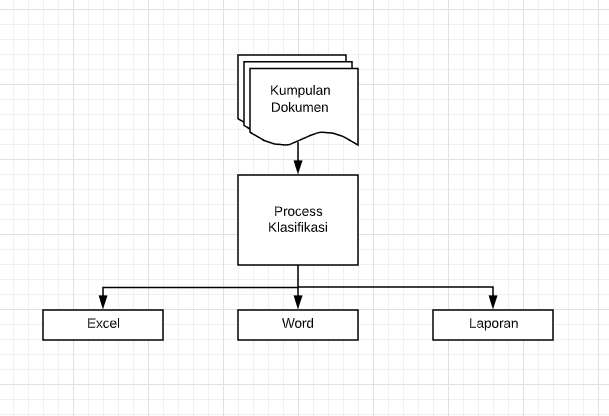
\includegraphics[scale=0.2]{figures/1174002/4/1.PNG}
\caption{contoh klasifikasi teks}
\label{contoh}
\end{figure}

\item Jelaskan mengapa klasifikasi bunga tidak bisa menggunakan machine learning, sertakan ilustrasi sendiri.\par
Klasisifikasi Bunga tidak dapat dimasukkan ke dalam mesin learning karena jenis-jenis bunga kebanyakan hampir mirip atau memiliki ciri ciri yang sama namun tidak mirip. Hal itu yang menyebabkan klasifikasi bunga tidak bisa digunakan oleh mesin learning.

\begin{figure}[ht]
\centering
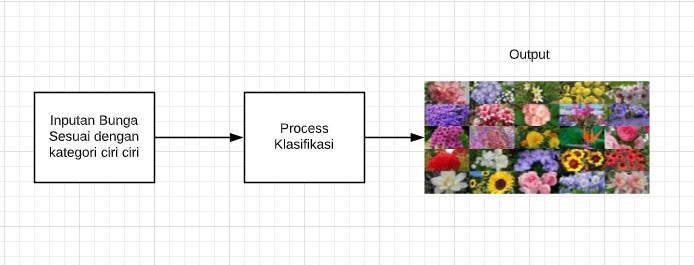
\includegraphics[scale=0.2]{figures/1174002/4/2.PNG}
\caption{contoh klasifikasi bunga}
\label{contoh}
\end{figure}

\item Jelaskan bagaimana teknik pembelajaran mesin pada teks pada kata-kata yang digunakan di youtube,jelaskan arti per atribut data csv dan sertakan ilustrasi buatan sendiri.\par
Cara Pembelajaran teks yang ada pada youtube yaitu dengan cara merekam jejak penelusuran yang sering dicari dan terakhir kali dicari sebelumnya, kita bisa melihat ini pada menu pencarian youtube dan history youtube. namun pada contoh dibawah ini menggunakan menu pencarian youtube untuk melihat teks yang terakhir kali dicari di youtube hanya dengan klik pada kolom pencarian.

\begin{figure}[ht]
\centering
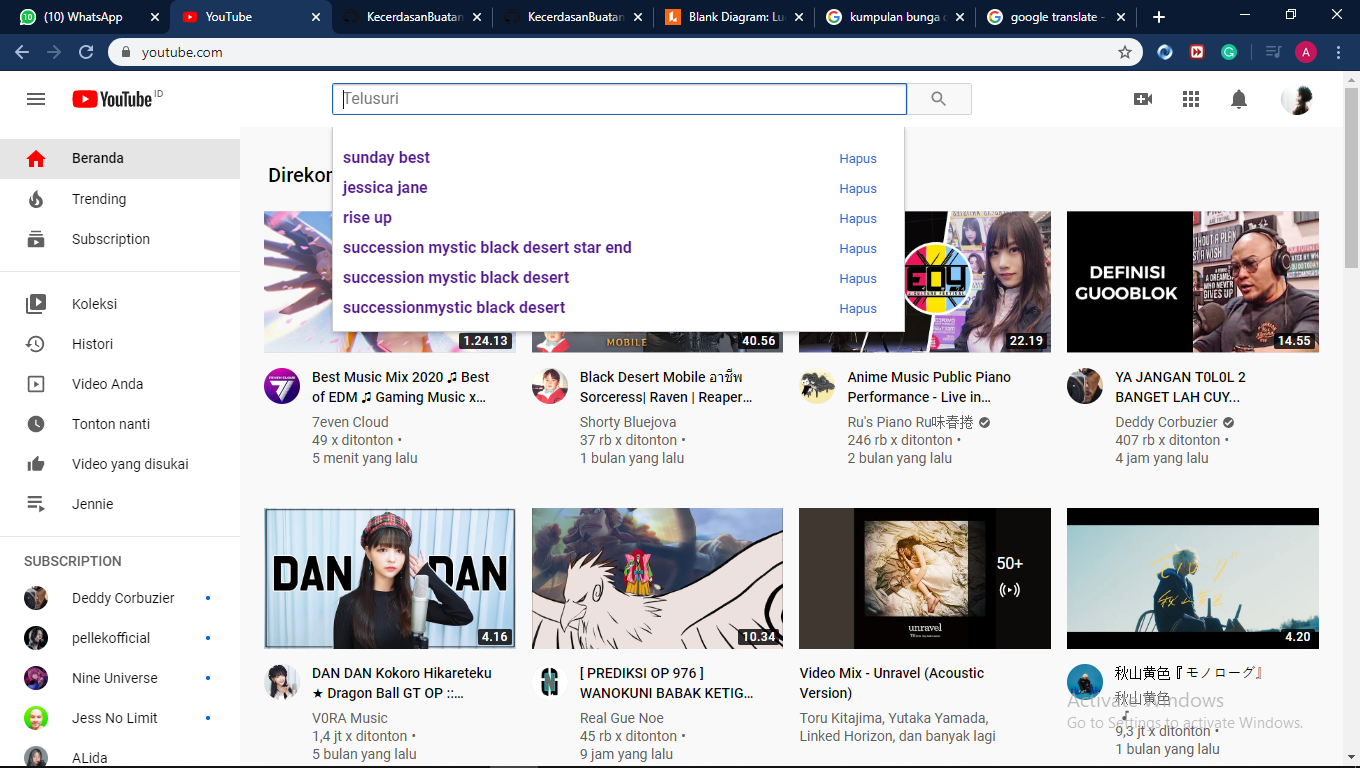
\includegraphics[scale=0.2]{figures/1174002/4/3.PNG}
\caption{contoh teknik pembelajaran mesin}
\label{contoh}
\end{figure}

\item Jelaskan apa yang dimaksud vektorisasi data.\par
vektorisasi data merupakan pemechan data menjadi bagian bagian yang lebih sederhana contoh pada satu paragraf terdiri dari 200 kata kemudian dilakukan vektorisasi dengancara membagi-bagi kata dalam paragraf tersebut ke dalam kalimat-kalimat yang terpisah kemudian di pecah lagi menjadi data dalam perkata selanjutnya kata kata tersebut di terjemahkan.

\item Jelaskan apa itu bag of words dengan kata-kata yang sederhana dan ilustrasi sendiri.\par
 bag of words merupakan peroses penyederhanaan kata-kata, Misalnya Satu kalimat diubah menjadi perkata dan dikelompokkan lalu akan dilakukan perhitungan frekuensi kemunculan setiap kata katanya.
\begin{figure}[ht]
\centering
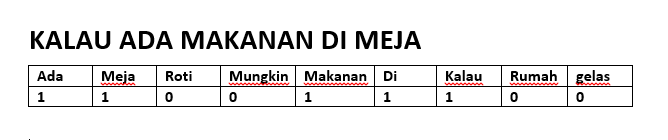
\includegraphics[scale=0.2]{figures/1174002/4/4.PNG}
\caption{contoh bag of words}
\label{contoh}
\end{figure}

\item Jelaskan apa itu TF-IDF, ilustrasikan dengan gambar sendiri.
 TF-IDF merupakan metode untuk menghitung bobot dari kata yang sering muncul pada suatu kalimat. metode ini menghitung nilai TF atau Term Frequency dan IDF atau Inverse Document Frequency pada setiap kata pada kalimat yang dijadikan acuan kata pada metode ini sering di sebut token.
 
\begin{figure}[ht]
\centering
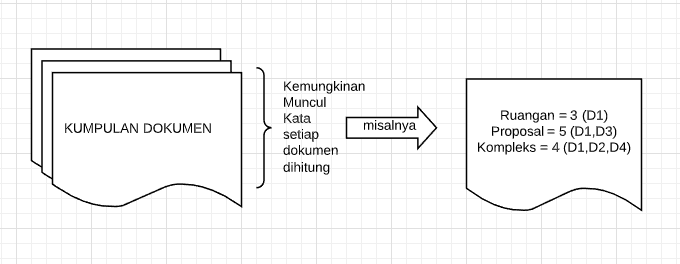
\includegraphics[scale=0.2]{figures/1174002/4/5.PNG}
\caption{contoh TF-IDF}
\label{contoh}
\end{figure}

\end{enumerate}


